\section{Motivation: from finite element to neural network}\label{FE2NN}
In this section, we will introduce the so-called shallow neural network 
(deep neural network with one hidden layer) from the viewpoint of finite element method.

Let us recall the linear finite element functions on the unit interval $\bar{\Omega}=[0,1]$ in Section \ref{linearFE}. 
Consider a set of equidistant girds $\mathcal T_\ell$ of level $\ell$ and mesh length $h_\ell = 2^{-\ell}$. The grid points $x_{\ell,i}$ are given by
\begin{equation}
x_{\ell,i}:=ih_\ell,\quad 0\le i\le 2^\ell.
\end{equation} 
For $\ell=1$, we denote the special hat function by $\varphi(x)$ and any nodal basis function in \eqref{1dbasis:function} on grid $\mathcal T_\ell$ by $\varphi_{\ell,i} $ as below
\begin{equation}\label{def_g}
\varphi(x) = 
\begin{cases}
2x \quad &x\in [0,\frac{1}{2}] \\
2(1-x) \quad &x\in [\frac{1}{2}, 1] \\
0, \quad &\text{others} 
\end{cases},\qquad
\varphi_{\ell,i} = \varphi(\frac{x - x_{\ell,i-1}}{2h_\ell}) = \varphi(w_\ell x + b_{\ell,i}).
\end{equation} 
That is to say, any $\varphi_{\ell,i}(x)$ can be obtained from $\varphi(x)$ by scaling 
(dilation) and translation with 
\begin{equation}\label{key}
w_\ell = 2^{\ell-1}, \quad b_{\ell,i} = \frac{-(i-1)}{2},
\end{equation}
in $\varphi_{\ell,i} = \varphi(w_\ell x + b_{\ell,i})$. 
\begin{figure}[H]
\centering
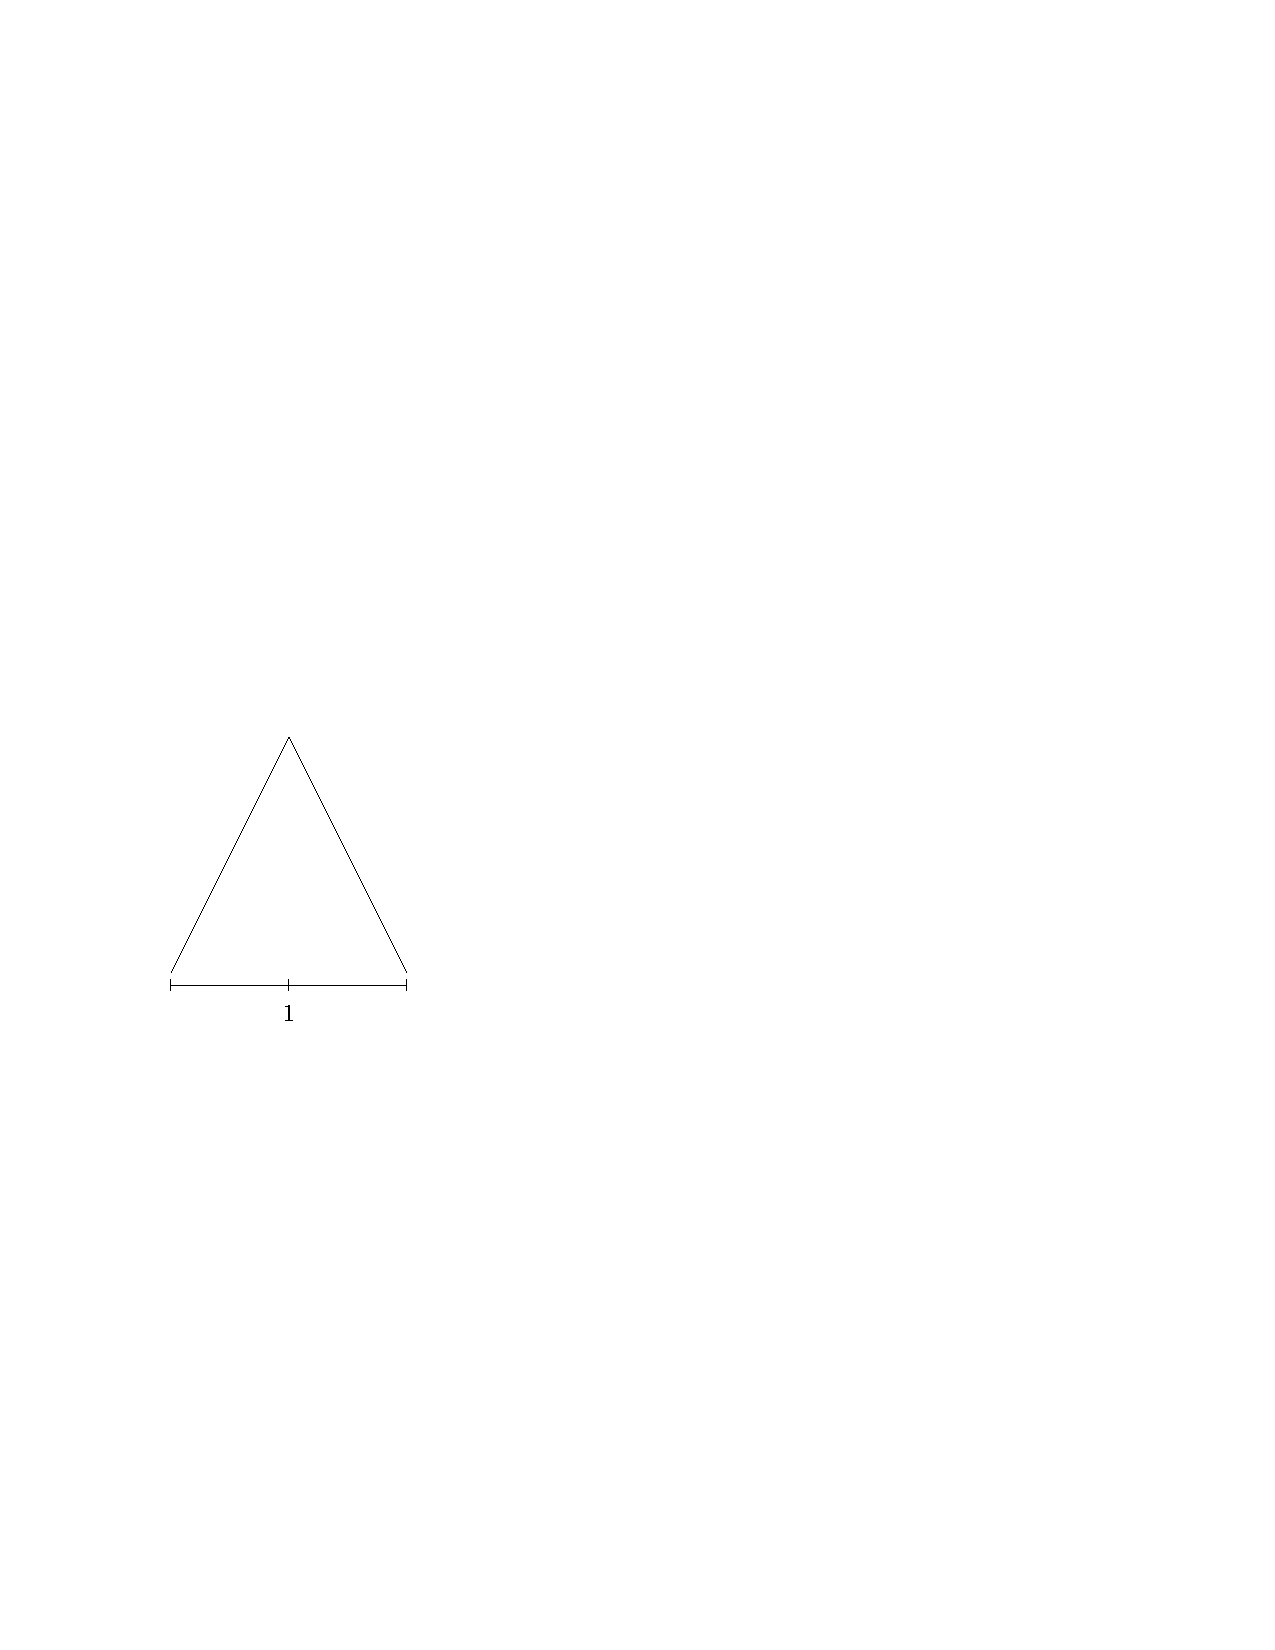
\includegraphics[width=4cm]{1dbasis1.pdf}\qquad
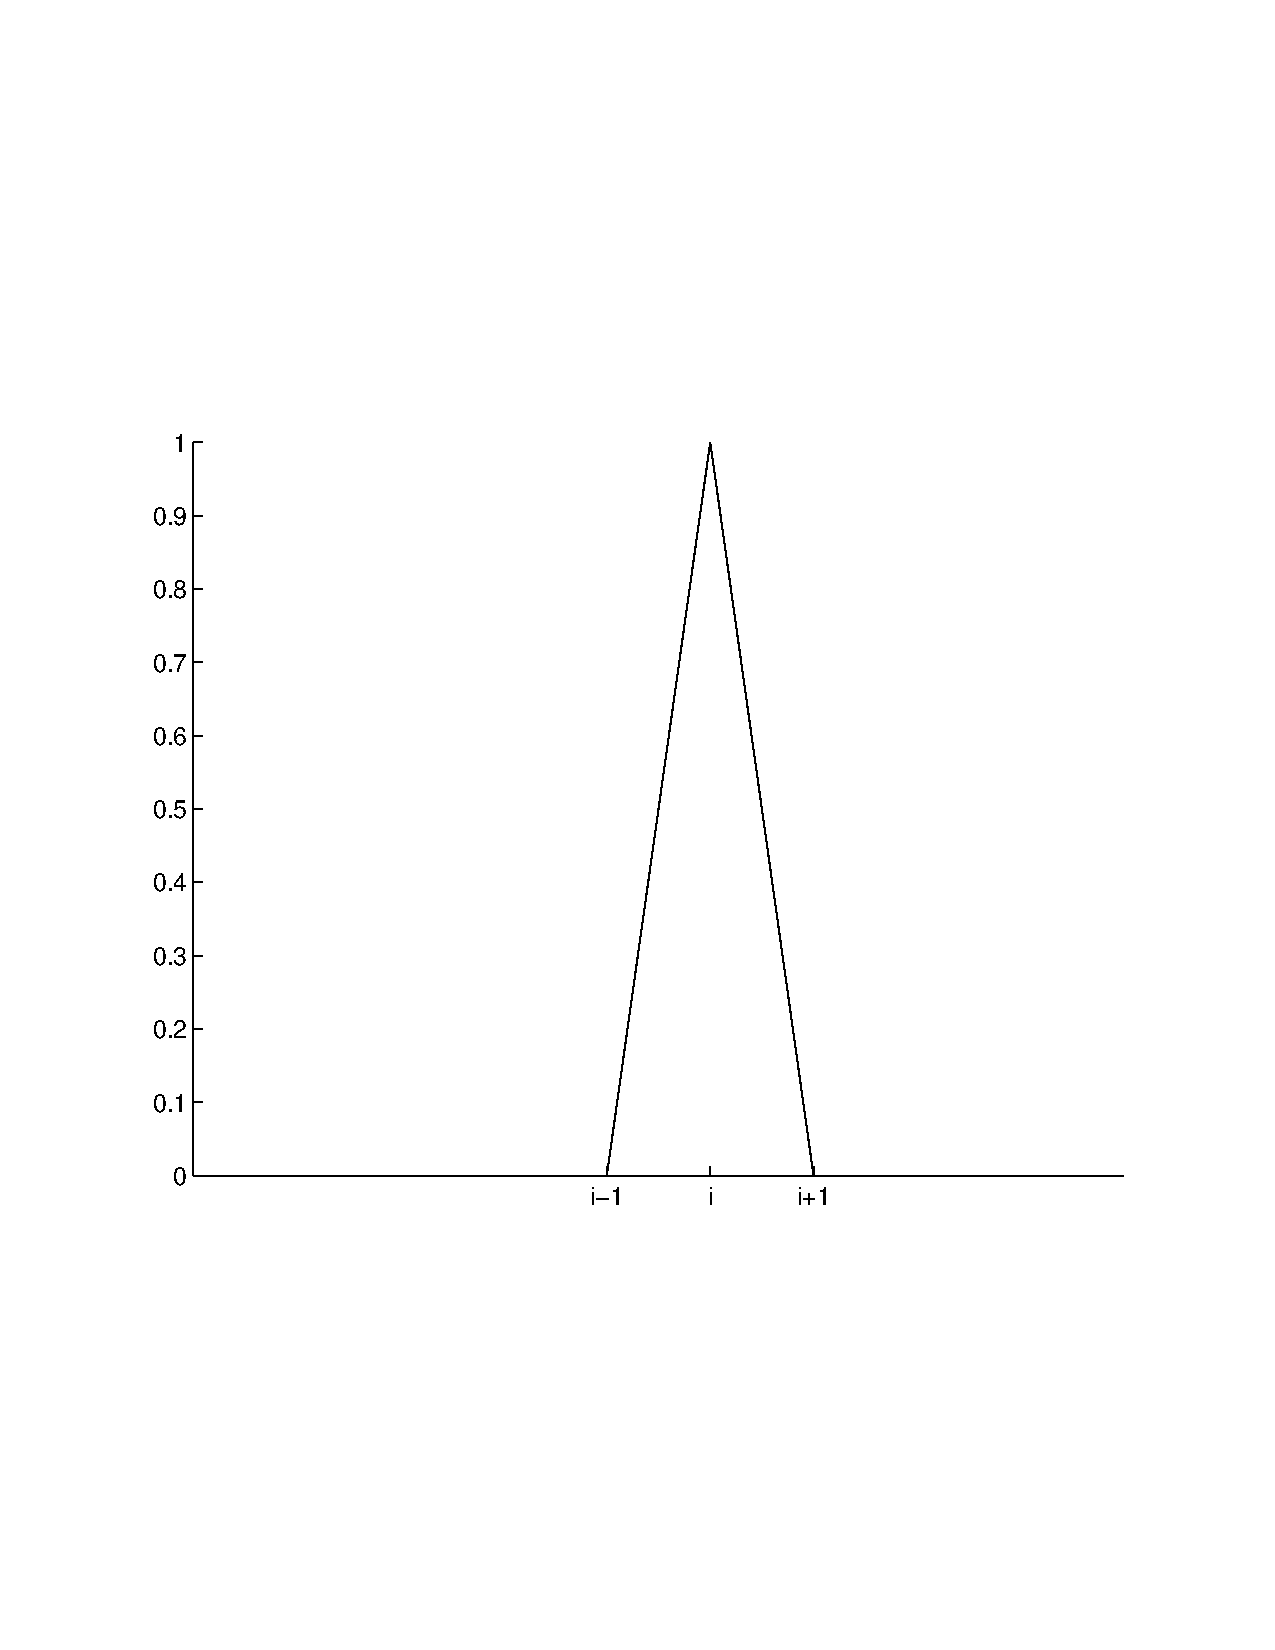
\includegraphics[width=5cm]{basisfunction.pdf}
\caption{Diagram of $\varphi(x)$ (left) and $\varphi_{\ell,i}(x)$ (right).}
\end{figure} 


Let us recall the finite element interpolation in Section \ref{linearFE} as
\begin{equation}\label{key}
u(x) \approx u_\ell(x) := \sum_{ 0\le i \le 2^\ell} u(x_{\ell,i}) \varphi_{\ell,i}(x),
\end{equation}
for any smooth function $u(x)$ on $(0,1)$. The above interpolation will converge as $\ell \to \infty$, which shows that
\begin{equation}\label{key}
{\rm span} \left\{  \varphi(w_\ell x + b_{\ell,i}) \right\} \quad \text{is dense in} \quad H^1(0,1).
\end{equation}
Thus, we may have the next concise relation:
\begin{equation}\label{key}
\begin{split}
\text{FE space} =  &{\rm span} \left\{  \varphi(w_\ell x + b_{\ell,i}) ~|~ 0\le i \le 2^\ell, \ell = 1, 2, \cdots \right\} 
\\
\subset  &{\rm span} \left\{  \varphi(w x + b) ~|~  w, b \in \mathbb{R} \right\}.
\end{split}
\end{equation}
In other words, the finite element space can be understood as the linear combination of $\varphi(w x + b)$ with certain special choice of $w$ and $b$. 

Here, we need to point out that this ${\rm span} \left\{  \varphi(w x + b) ~|~  w, b \in \mathbb{R} \right\}$ is exact the deep neural networks with one hidden layer (shallow neural networks) with activation function $\varphi(x)$. More precisely, 
\begin{equation}\label{key}
f \in {\rm span} \left\{  \varphi(w x + b) ~|~  w, b \in \mathbb{R} \right\},
\end{equation}
means there exist positive integer $N$ and $w_j, b_j \in \mathbb{R}$ such that 
\begin{equation}\label{key}
f = \sum_{j=1}^N a_j \varphi(w_j x + b_j),
\end{equation}
which is also called one hidden neural network function with $N$ neurons.

\begin{remark}
	\begin{enumerate}
		\item By making $w_\ell$ and $b_{\ell,i}$ in \eqref{def_g} arbitrary, we get a much larger class of 
		function which is exact a special neural network with activation function $\varphi(x)$.
		\item Generalizations: 
		\begin{enumerate}
			\item activation function $\varphi$ can be different, such as ${\rm ReLU}(x) = \max\{0,x\}$.
			\item There is a natural extension for high dimension $d$ as
			\begin{equation}\label{key}
			\left\{  \varphi(w\cdot x + b) \right \},
			\end{equation}
			where $w\in \mathbb{R}^d$, $b\in \mathbb{R}$ and $\displaystyle w\cdot x = \sum_{i=1}^d w_i x_i$.
			This is called ``deep'' neural network with one hidden layer.
		\end{enumerate}
	\end{enumerate}
\end{remark}


%\input{3FEM/2dFEM}
